\documentclass[11pt,a4paper]{article}

\usepackage[margin=2.3cm]{geometry}
\usepackage{amsmath,amssymb}
\usepackage{graphicx}
\usepackage{booktabs}
\usepackage{xcolor}
\usepackage{enumitem}
\usepackage[hidelinks]{hyperref}
\usepackage{caption}

\emergencystretch=1.5em
\captionsetup{font=small,labelfont=bf,width=.92\textwidth}
\setlength{\parskip}{4pt plus 1pt}
\setlength{\parindent}{0pt}

\newcommand{\code}[1]{\texttt{#1}}
\newcommand{\dv}[1]{diverged (#1)}

\title{Effect of the kappa correction in RBLapSum\\[2pt]
\large Research note: \code{through\_rank\_kappa} versus plain
\code{through\_rank} at $b_0=0$}
\author{}
\date{2026-09-21.}

\begin{document}
\maketitle
\vspace{-2em}

% ============================================================
\section{Purpose and summary of conclusions}
% ============================================================

RBLapSum's boundary surrogate can be applied in two forms. In plain
\code{through\_rank}, each candidate's score gradient is the
kernel-weighted boundary term itself. In \code{through\_rank\_kappa}, the
same term is additionally passed through the LapSum rank-one Jacobian at
the boundary,
\[
g = a - q\,{\textstyle\sum_i a_i},\qquad q_i=\kappa_i/{\textstyle\sum_j \kappa_j},
\]
which removes the common score-translation mode. This note tests whether
the kappa correction improves convergence, using matched training runs at a
boundary floor of $b_0=0$ (the new default; the earlier campaigns used
$b_0=0.1$).

Conclusions:

\begin{itemize}[leftmargin=1.4em]
\item \textbf{The kappa correction is decisively better in every tested
configuration.} Plain \code{through\_rank} diverges within the first
$\sim$1700 steps in all four configurations with $K\geq 64$, and in the two
$K=32$ configurations where it survives it converges $0.085$--$0.164$ nats
worse than \code{through\_rank\_kappa} while showing repeated large
excursions along the way.

\item \textbf{With the correction, five of six configurations converge},
at final validation CE $1.46$--$1.55$; the exception is $(K,J)=(64,64)$ at
$T=1$, which diverged at step 8680. The $K=64$, $T=1$ row is the known
marginal row of this surrogate.

\item \textbf{The boundary floor does not matter in these regimes.} The
four \code{through\_rank\_kappa} configurations that were previously
trained at $b_0=0.1$ reproduce at $b_0=0$ within $\pm0.005$ nats, in line
with the earlier measurement that the mean boundary stays $8$--$40\times$
above the old floor.
\end{itemize}

% ============================================================
\section{Setup}
% ============================================================

Twelve runs, all under full magnitude--direction decoupling with the same
architecture, data, optimizer, schedules, and seed as the concurrent
MD-versus-MD-init campaign (8$\times$768, \code{abs\_topk} over $N=1536$,
\code{residual\_out}, batch $96\times512$, 20k steps). The grid pairs the
two gradient modes at
\[
(K,J,T)\in\{(32,32,1),\,(32,480,1),\,(64,64,1),\,(64,448,1),\,
(128,128,2),\,(128,384,2)\},
\]
with $T=2$ for the $K=128$ rows because $K=128$, $T=1$ is known to diverge
under every regime. All runs use $b_0=0$; the run names carry a
\code{b00} marker. Divergence is detected and the run stopped by the same
guard as in the companion note (non-finite CE, or CE far above its own best
for a sustained window).

% ============================================================
\section{Results}
% ============================================================

\begin{center}\small
\begin{tabular}{llcc}
\toprule
$(K,J)$ & $T$ & \code{through\_rank\_kappa} & \code{through\_rank} \\
\midrule
$(32,32)$   & 1 & 1.5533 & 1.6382 \\
$(32,480)$  & 1 & 1.4918 & 1.6558 \\
$(64,64)$   & 1 & \dv{8680} & \dv{1580} \\
$(64,448)$  & 1 & 1.4776 & \dv{1620} \\
$(128,128)$ & 2 & 1.4792 & \dv{1580} \\
$(128,384)$ & 2 & 1.4615 & \dv{1680} \\
\bottomrule
\end{tabular}
\end{center}

Final validation CE after 20k steps, or the step at which the run was
stopped as diverged.

\begin{figure}[h]\centering
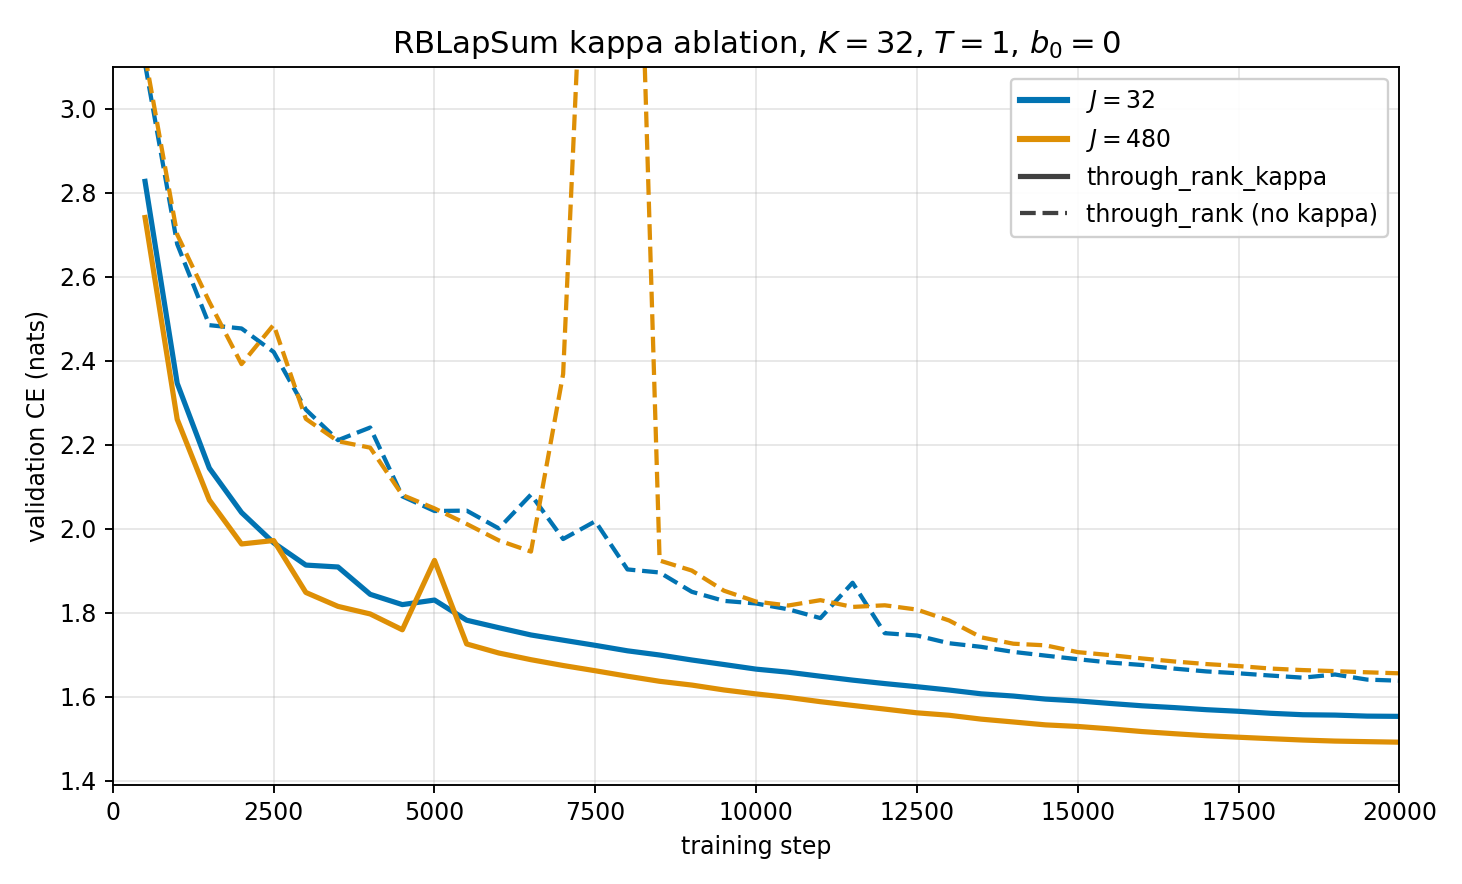
\includegraphics[width=.82\textwidth]{figures/kappa_val_k32.png}
\caption{$K=32$, $T=1$: both modes survive. The plain
\code{through\_rank} runs (dashed) sit $\sim$0.1 nats above their kappa
counterparts throughout training and undergo repeated large excursions,
including a recovered burst of the $J=480$ run around steps
7000--8500.}
\end{figure}

\begin{figure}[h]\centering
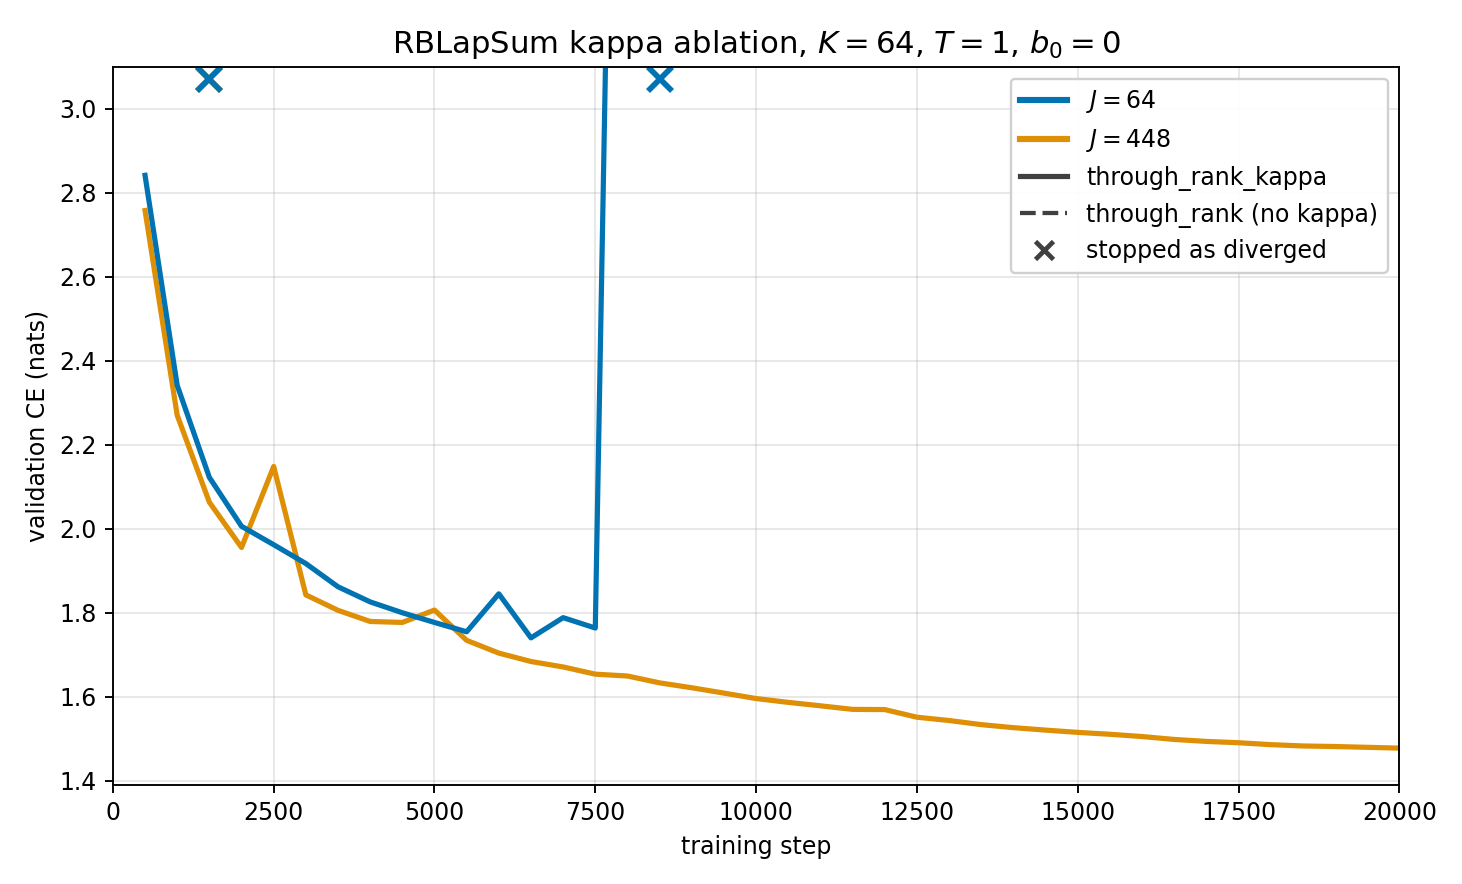
\includegraphics[width=.82\textwidth]{figures/kappa_val_k64.png}
\caption{$K=64$, $T=1$: both \code{through\_rank} runs diverge within the
first $\sim$1600 steps (crosses at the top edge). With the kappa
correction, $J=448$ converges to $1.4776$ while $J=64$ survives to step
8680 before a terminal burst.}
\end{figure}

\begin{figure}[h]\centering
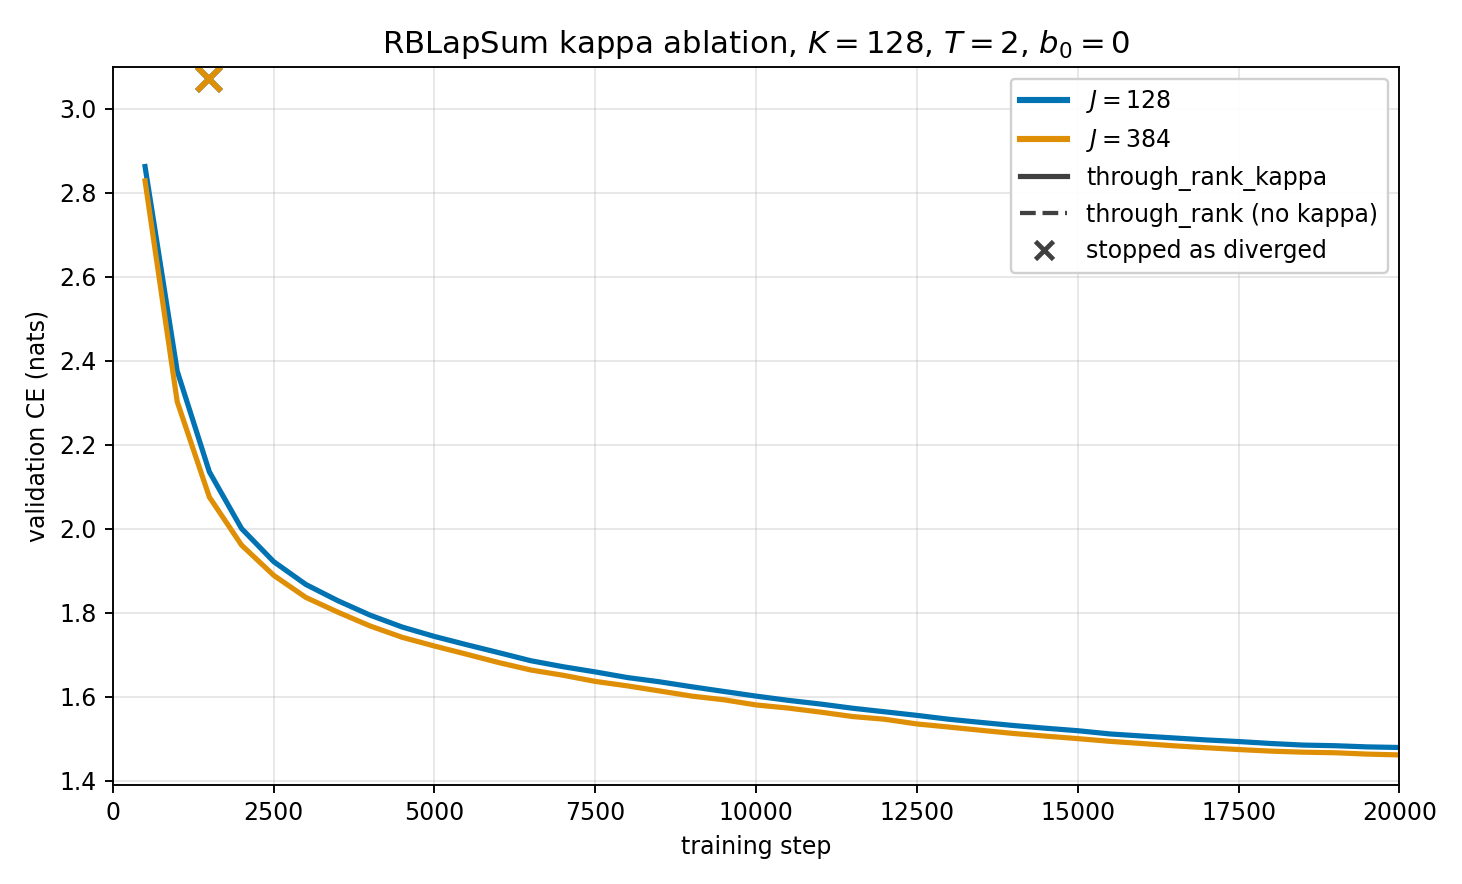
\includegraphics[width=.82\textwidth]{figures/kappa_val_k128_t2.png}
\caption{$K=128$, $T=2$: both \code{through\_rank} runs diverge within the
first $\sim$1700 steps; both kappa runs converge.}
\end{figure}

\textbf{Comparison with the earlier $b_0=0.1$ runs.} Four of the kappa
configurations have direct twins in the MD-versus-MD-init campaign, which
ran at $b_0=0.1$ but is otherwise identical:

\begin{center}\small
\begin{tabular}{llccc}
\toprule
$(K,J)$ & $T$ & $b_0=0.1$ & $b_0=0$ & difference \\
\midrule
$(32,32)$   & 1 & 1.5482 & 1.5533 & $+0.0051$ \\
$(32,480)$  & 1 & 1.4923 & 1.4918 & $-0.0005$ \\
$(128,128)$ & 2 & 1.4778 & 1.4792 & $+0.0014$ \\
$(128,384)$ & 2 & 1.4602 & 1.4615 & $+0.0013$ \\
\bottomrule
\end{tabular}
\end{center}

The differences are within run-to-run noise, confirming that the earlier
results were not shaped by the floor.

One historical contrast is worth recording: at $(K,J)=(64,448)$, $T=1$,
the original $b_0=0.1$ campaign run destabilized near step 3940, while the
present $b_0=0$ run converged cleanly. Given the four replication pairs
above, this should be read as the known run-to-run stochasticity of
divergence in a marginal row rather than as an effect of the floor; the
same row also splits here between its $J=448$ survivor and its $J=64$
death.

% ============================================================
\section{Conclusion}
% ============================================================

The kappa correction is not an optional refinement of the
\code{through\_rank} surrogate; in these setups it is what makes the
surrogate usable. Without it, training survives only in the most
conservative row tested ($K=32$, $T=1$), and even there at a
$0.085$--$0.164$ nat penalty with visibly bursty dynamics. With it, every
configuration except the marginal $(64,64)$, $T=1$ cell converges to
$1.46$--$1.55$. All cells are single runs at one seed, so individual
divergences carry the usual stochastic caveat; the mode-level separation,
however, is uniform across all six configurations.

\end{document}
